\documentclass[a4paper,10pt]{report}
\usepackage{graphicx}
\usepackage[procnames]{listings}
\usepackage{amsmath}
\usepackage[utf8]{inputenc}
\renewcommand{\baselinestretch}{1.55}
\renewcommand{\bibname}{References}
% Title Page
\title{\textbf{Anti-Theft Tracking and Location Detection}}
\author{\textbf{Project By:}\\Aditya Landge(101228)\\Rohan Manudhane(101231)\\Chinmay Lad(101226)\\[0.3in]\textbf{Project Guide:}\\Rakhi Kalantri}


\begin{document}
\maketitle
\tableofcontents

\chapter{Introduction}
In today’s world of revolutionary innovative technology various gadgets that can fit our pockets for everyday use are manufactured and made available at low rates. With the technology becoming cheaper, more people use different devices on a much larger scale with an exponential increase in the rate of sales. These days it’s very common for a person to own mobile phones, cars and other valuable tech items. However these gadgets and items like mobile, purses, wallets, bags, etc become easy target for thieves to steal them. With the increase in the robbery and such crimes it is very important to contain it. Gone are the traditional days of searching stolen items, with the techno-boom there is also increased intelligence available in the field of security which should be harnessed.Hence, using this motivation to try and contain these robberies and actually recover the stolen item we introduce the idea of ATTLD (Anti-Theft Tracking and Location Detection Chip).\\[0.15in]
ATTLD is a GPS tracking device that when installed in a device can provide its location and give the information to the owner (via website). The latest tracking devices make use of GPS. The additional feature ATTLD has is that it can communicate with other ATTLDs in its proximity and make the owner of the device aware of the location. All the owner has to do is to go to the site and flag his device as stolen so that other ATTLDs are aware of the stolen device. This makes the location of object a relatively simpler task.If the device with the chip on it gets stolen then the location I.D is sent to the company which then sends alert messages to all the other devices in the vicinity.All the other chips of the vicinity will start searching the particular chip with the I.D and as soon as any chip finds the chip in question then the location is found of the stolen device which can then be retrieved.
The aim of this project is to develop a means of communication by which the stolen object can be tracked.

\chapter{Application}
\begin{itemize}
 \item This project can be used in Cars, public and private buses, even in bikes and motorcycles.
 \item ATT can be used in various schools which have buses or vans for their student’s security.
 \item This can be used in supermarkets, shopping malls and libraries.
 \item By using the Application, you can easily locate the device's location.
\end{itemize}


\chapter{Literature Survey}
\begin{itemize}
  \item \textbf{Bike Tracking:}\\Tracking Stolen Bikes through Everyday Mobile Phones and Participatory Sensing [6][10]. The study presents a participatory sensing system that uses everyday smartphones and low-cost Bluetooth devices to help people recover their bikes by maintaining the location log periodically.
  \item \textbf{Anti-Car Theft System using Android Phone:}[1][10]\\The paper presents anti-car theft system that uses everyday smartphones and bluetooth devices to help people to track their cars.
  \item \textbf{Bluetooth an Optimal Solution for Personal Asset Tracking:}[3][8]\\This study compares the Tracking Technologies including Bluetooth and RFID and gives us an insight on various factors of communication and provides us pros and cons of the various technologies.
  \item \textbf{Wi-Fi Tracker:}\\An Organization Wi-Fi Tracking System[4]. This paper presents Tracking Technologies for organization which has Wi-Fi.
\end{itemize}
\chapter{Scope}
The utility model is a Bluetooth anti-theft, anti-lost location detection and tracking chip called as ATT. The ATT is using the following protocol: It contains the Bluetooth chip, LED lights, speaker and/or micro vibration motor, battery. The Bluetooth chip includes a transmitter and receiver components member,
the LED lights are battery powered and are used for easy detection of device (with respect to visibility of device) in case it is misplaced or in absence of visible light, the speaker and/or micro vibrator motor too are battery powered and serve the same functions as the LED lights and will be used to detect the device with sound waves as the medium.
The ATT is Bluetooth anti-theft, anti-lost location detection and tracking chip and is installed on various mobile devices and accessories like mobile phone sets, tablets, watches, key chains, etc. The Bluetooth chip in ATT device transmits and receives information with a mobile phone having the application installed in it. Each ATT device will have an independent verification scheme to synchronize with the Smartphone Application.\\
\newpage
The chip is will be designed to serve two main purposes (scenarios):
\begin{itemize}
\item \textbf{To detect a misplaced object:}\\In this case the person has misplaced his/her gadget in the vicinity for example in a room, the device’s Bluetooth communication, communicates with the user’s Smartphone and the user is able to find the device on the basis of the Bluetooth signal strength.
\item \textbf{To track and find a lost object:}\\In this case the person has lost the device or the device has been stolen and the ATT is not in user’s Smartphone’s range. This is the case where the user has to just tag the device as stolen on the website and the server will list the ATT device as lost and sends this information to all the ATT users with the app installed and keeps their phone on lookout for the lost.
\end{itemize}
\chapter{Proposed System}
Following are some of the functionalities of Proposed System:
\begin{itemize}
 \item User can make ATT buzz, sound or flash LED’s by pressing the button in the Application from your Smartphone to detect the mobile device or gadget to which ATT is attached.
 \item By pressing the detection key in your ATT device provision will be made to detect the Smartphone to which the ATT device is synchronized with.
 \item ATT will sound, vibrate and flash LED’s automatically when about 10 meters away from your Smartphone .i.e. it will indicate that the ATT device is moving out of the Bluetooth range of the Smartphone.
\end{itemize}
If you mark an item as lost the entire ATT community of users will anonymously and securely help you find your ATT. This essentially expands your reach in finding your device. The more family and friends in the community, better the capability. ATT’s can be designated to easily discover which of your friend ATTs is closest to your lost.\\
\newpage
The system is divided into 2 basic parts called Scenarios:
\section{First Scenario:}
In the first scenario, gadget location on which the device is mounted is found out by the strength of the signal between the smartphone and the ATT chip. As the chip is in the vicinity it can be connected to the smartphone and based on the signal strength the user could be able to navigate to the gadget. This is done by receiving the RSSI[5][9] value. The RSSI value returns the signal strength between the devices. When the distance between the devices increase the RSSI value drops down and accordingly the user is indicated that the signal strength is decreased. Therefore when the user goes in one direction for searching the gadget he/she will see the signal strength, if the signal strength drops the the device is not in the direction they are going and thus can change the direction. Eventually the user reaches the gadget as the signal goes on strengthening.\\[0.3in]
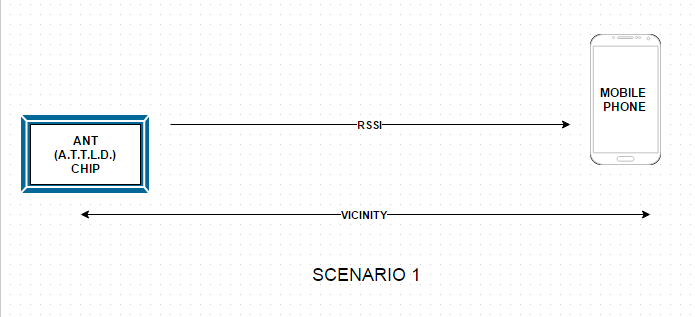
\includegraphics[scale=0.7]{images/scenea}
\newpage
\section{Second Scenario:}
In the second scenario, to find out the gadget location is much complicated. The gadget in not in the vicinity and thus cannot be connected to the ATT Chip. If the user is not able to find it, then he/she can go upto the web server and tag the device as stolen. Tagging the device as stolen put the device in the search list and this search list is updated in smartphones that have the ANT App. Thus when the stolen chip comes in contact with any of the smartphone the smartphone sends it location to the server and the corresponding owner of the chip is informed. This works in the following manner the list of devices which are tagged lost or stolen are updated to all the smartphones containing the ANT app. When the stolen chip is in the vicinity of the smartphone app, the smartphone immediately send its GPS[7] coordinates to the server. Based on the coordinates received server maps the location and the user is notified the user then can untag the device from the list or if the device is not found at the location the user may leave the tag on the device and let other smartphones find the chip. The proposed work would be to analyse various parameters mentioned above by changing the existing setup.\\[0.3in]
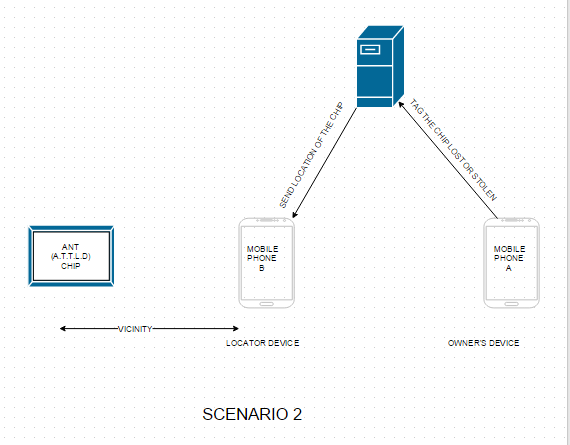
\includegraphics[scale=0.7]{images/sceneb}
\newpage
\addcontentsline{toc}{chapter}{References}

\begin{thebibliography}{9}
 \bibitem{anticartheft}
 Jake M. Laguador, Moulle M. Chung, Frina Joy D. Dagon, Julie Ann M. Guevarra, Rommel J. Pureza, Jeffrey D. Sanchez, and Dan Kenneth I. Sta. Iglesia, Anti Car Theft System using Android Phone, International Journal Of Multidisciplinary Sciences And Engineering, Vol. 4, No. 5, June 2013.
 \bibitem{threats}
 Nateq Be-Nazir Ibn Minar, and Mohammed Tarique ,Bluetooth Security Threats And Solutions: A Survey, International Journal of Distributed and Parallel Systems (IJDPS) Vol.3, No.1, January 2012.
 \bibitem{comparison}Dr. Saleem Ahmad, Ruoyu Lu, Muhammad Ziaullah, Bluetooth an Optimal Solution for Personal Asset Tracking: A Comparison of Bluetooth, RFID and Miscellaneous Anti-lost Traking Technologies, International Journal of u- and e- Service, Science and Technology 03/2015; Vol:8(No.3):179-188. DOI: 10.14257/ijunesst.2015.8.3.17
 \bibitem{wifitrack}I. A. Mingkhwan, Wi-Fi Tracker: An Organization Wi-Fi Tracking System, In Proceedings f Canadian Conference On Electrical And Computer Engineering Ccece '06.
 \bibitem{embeded}Wilson M. Yeung, Joseph K. Ng, “Wireless LAN Positioning based on Received Signal Strength from Mobile device and Access Points”, in Proceedings of 13th IEEE International Conference on Embedded and Real-Time Computing Systems and Application, RTCSA’07.
 \bibitem{biketrack}Ted Tsung-Te Lai, Chun-Yi Lin, Ya-Yunn Su, and Hao-Hua Chu  BikeTrack: Tracking Stolen Bikes through Everyday Mobile Phones and Participatory Sensing www.csie.ntu.edu.tw/\~yysu/BikeTrack\_ phonesense11.pdfo
 \bibitem{foo} Guha, S., Plarre, K., Lissner, D., and Bhagavathy Krishna, S. M., Dutta, P., and Kumar, S. Autowitness: Locating and tracking stolen property while tolerating gps and radio outages, In SenSys, 2010
 \bibitem{bar}. Dawson, “Device Tracking on a Scattered Bluetooth-Enabled Network”, Bsc Dissertation, Faculty of Engineering, University of Bristol, May 2005
 \bibitem{foobar} A, Frunzke T and Dressler F, 2007, Adaptive Distance Estimation and Localization in WSN using RSSI Measures. In: Proceedings of the 10th Euromicro Conference on Digital System Design Architectures, Methods and Tools, 471-478
 \bibitem{foobarr}Rohitaksha K , Madhu C G , Nalini B G ,Nirupama C V .Android Application for Vehicle Theft Prevention and Tracking System, Rohitaksha K et al, / (IJCSIT) International Journal of Computer Science and Information Technologies, Vol. 5 (3) , 2014, 3754-3758
\end{thebibliography}

\end{document}          
